%%%%%%%%%%%%%%%%%%%%%%%%%%%%%%%%%%%%%%%%%%%%%%%%%%%%%%%%%%%%%%%%%%%%%%%%
\chapter{Neuartige modellbasierte Teststrategie für große agile Projekte}
\label{sec:results}
%%%%%%%%%%%%%%%%%%%%%%%%%%%%%%%%%%%%%%%%%%%%%%%%%%%%%%%%%%%%%%%%%%%%%%%%

Aufbauend auf den Erkenntnissen der Fallstudie (siehe Abschnitt \ref{sec:fallstudie}) wurde eine neuartige modellbasierte Teststrategie entwickelt um komplexe Softwaresysteme in agilen Projekten zu testen. Diese Strategie hat unter anderem folgende Eigenschaften und zielt auf die, in Abschnitt \ref{sec:schwachstellen_raiffeisen}, beschriebenen Schwachstellen ab:

\begin{enumerate}
\item Einfachere Einbindung der Fachbereiche und Minimierung der Spezifikations-/Implementationslücke.
\item Minderung des Wartungsaufwandes für die Testlogik
\item Eliminierung der Notwendigkeit eine hohe Anzahl von einzelnen Teställen zu definieren
\item Visualisierung der Spezifikation und Bewusstmachung des potenziellen Testaufwandes
\item Minimierung der Abhängigkeit zu einem Werkzeug durch Wahl eines quelloffenen Tools
\item Möglichkeit des punktuellen Einsatzes bzw. der inkrementellen Einführung
\item Erhöhung der Testabdeckung und damit Erhöhung der Qualität des Softwaresystems
\end{enumerate}

Im folgenden wird die genannte Teststrategie näher beschrieben. Abbildung \ref{fig:testarchitektur} stellt die Testarchitektur konzeptuell dar.

\begin{figure}[h] 
  \centering
     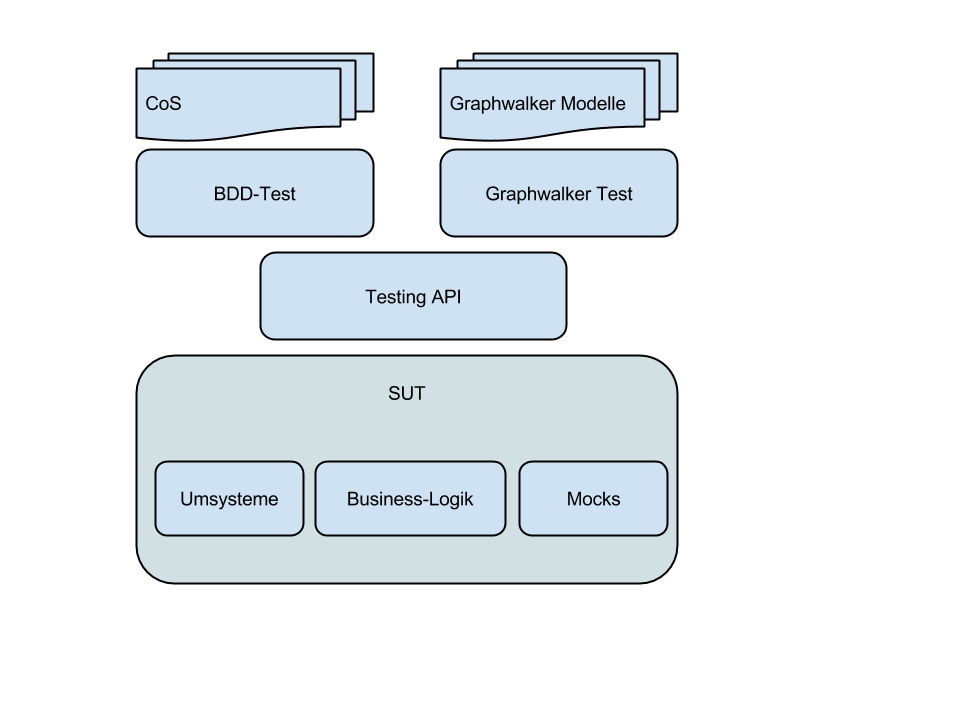
\includegraphics[width=1.0\textwidth]{figures/Testarchitektur-MBT-BDD-COS.png}
  \caption{Am oberen Ende der Testarchitektur liegen die \textit{Conditions of Satisfiction}, die vom Kunden oder Fachbereich definiert werden. Sie dienen als Basis für die BDD-Tests. Graphwalker operiert auf Modellen im graphml-Format. Dabei können beide Frameworks entweder auf die Testing API zugreifen oder direkt auf das SUT.}
  \label{fig:testarchitektur}
\end{figure}

\section{Aufbau der Teststufen}
Im Sinne von Test-First und einer hohen Priorisierung von Unit-Tests soll der Fokus des Testings auf drei Arten von Tests liegen:

\begin{itemize}
\item Eine breite Basis von Unit-Tests mit hoher Abdeckung
\item Modellbasierte Systemtests auf mehreren Ebenen mit direkter Verbindung zu Anforderungen/Changes
\item Manuelle System- und Abnahmetests
\end{itemize}

In Anlehung an Linz\cite{linz_testing_2014} (und mit dem Verweis auf die Diskussion in Abschnitt\ref{sec:discussion_unit}) soll die Unit-Test Ebene in Scrum-Projekten am breitesten sein\todo{Test PYRAMIDE einfügen}. Dies erscheint mit Hinblick auf die vielen kurzen Iterationen, die das Softwaresystem stark verändern, auch logisch. Unit-Tests lassen sich, weil sie am entwicklungsnächsten sind, auch am schnellsten modifizieren. Obwohl Unit-Tests einzelne Komponenten in Isolation testen, müssen sie zumindest eine verlässliche Aussagen treffen können, dass ebenjene Komponente ordnungsgemäß operiert. Diese Aussage wird möglich durch eine hohe Codeüberdeckung in Verbindung mit sorgfältig designten Testfällen. Auch auf Unit-Testebene gelten Best-Practices und Methodiken für hochqualitative Testfälle, wie sie Spillner und Linz beschreiben\cite{spillner_software_2014}. Die Besonderheit im Unit-Testing dieser Teststrategie liegt im Einsatz eines Behaviour-Driven-Testing\cite{chelimsky_rspec_2010} Frameworks und einer Testing-API. Für erstere Komponente existieren einige frei erhältliche Vertreter\footnote{Im Java-Umfeld bekannt sind die Frameworks \textit{jBehave} \url{http://jbehave.org/} und \textit{cucumber} \url{https://cucumber.io/}}. In der Raiffeisen-Fallstudie wurde aber eine Eigenentwicklung als \textit{Proof of Concept} gemacht (siehe Abschnitt \ref{sec:bdd} für eine kurze Erläuterung). Die erwähnte Testing-API (siehe Abschnitt \ref{sec:testing_api}) bietet Schnittstellen zu Programmlogik und Umsystemen.\\
Im Sinne dieser Arbeit steht der modellbasierte Anteil der Teststrategie im Mittelpunkt. Es soll aber erwähnt sein, dass keine zwei Softwareprojekte gleich sind und sich die Gewichtungen der Testmethodiken im Detail unterscheiden \textit{sollten}! Der modellbasierte Anteil basiert technisch ausschließlich auf quelloffenen Werkzeugen. Graphwalker (die Funktionsweise des Graphwalker-Frameworks wird in Abschnitt \ref{sec:graphwalker} erklärt) funktioniert als Testtreiber der das SUT systmatisch durchläuft. Welche bzw. welche Art von Schnittstellen in das SUT greifen und es bedienen bleibt völlig offen und muss an die eigenen Bedürfnisse angepasst werden. Bei Applikationen mit GUI (oder wenn über die GUI \textit{End-to-End} Tests gemacht werden sollen) dann könnte zum Beispiel Selenium\footnote{Webseite des Selenium-Projekts \url{http://www.seleniumhq.org/}} eingesetzt werden. Tests auf Schnittstellenebene könnten durch SoapUI\footnote{ Offizielle Webseite von SoapUI \url{http://www.soapui.org/}} oder REST-assured\footnote{Code-Repository von REST-assured \url{https://code.google.com/p/rest-assured/}} angetrieben werden. Auch mächtigere proprietäre Werkzeuge können als Teil dieser Graphwalker-Teststrategie verwendet werden, sofern sie eine Schnittstelle zum Aufruf aus Java-Code besitzen und die Ergebnisse in irgendeiner Art und Weise (bevorzugt als JUnit-Report) zurückliefern können (dieser Ansatz wurde in der Fallstudie nicht erprobt und wird deshalb nicht näher erläutert). Außerdem können Graphwalker-Modelle nicht nur Workflows darstellen die auf GUI-Ebene ablaufen. Genauso vorstellbar sind Operationen die auf Schnittstellenebenen passieren (z.B. Operationen auf Datenbanken oder Web-Services). Bei solchen Tests macht es Sinn eine stabile Zwischenschicht, die Testing-API, einzubauen die wiederrum auf die darunterliegenden Systeme zugreift. Der Aufwand zur Erstellung der API rechtfertigt sich weil auch BDD-Unit-Tests darüber in das SUT greifen.\\
Zuletzt bleiben aber auch manuelle Tests ein wichtiger Bestandteil der Teststrategie. Einerseits sind das Abnahmetests bei Neuentwicklungen beziehungsweise bei modifizierten Teilen des Systems und andererseits auch Regressionstests die geschäftskritische Teile des Systems überwachen.

\section{Details der Teststrategie und Architektur}

\subsection{Behavior Driven Testing Framework}
\label{sec:bdd}
Der Fokus dieser Arbeit liegt auf dem modellbasierten Teil der Teststrategie, trotzdem soll erläutert werden welche Rolle \textit{Behavior Driven Testing} im Gesamtbild spielt. In der Softwareentwicklung, und vor allem in großen Projekten, wird viel Aufwand betrieben um Anforderungen von Domänenexperten möglichst nahtlos in die Implementation einfließen zu lassen. Abhängig vom Projekt liegen zwischen diesen Anforderungen und der endgültigen Realisierung mehrere Stufen und Parteien. Die Einführung von BDT zielt also vor allem auf die bereits erwähnte Minimierung der Spezifikations-/Implementationslücke. Auch MBT optimiert diesen Umstand (wie in Abschnitt \ref{sec:mbt_vorteile} beschrieben), aber es hat sich herausgestellt, dass es nicht zielführend ist für jede Anforderung den modellbasierten Ansatz anzuwenden.\\
Behavior Driven Testing, im weiteren Sinne bekannt als Behavior Driven Development, wurde ursprünglich von Dan North beschrieben. Er publiziert und diskutiert über BDD auf einer von ihm verwalteten Webseite\cite{north_official_2015}. BDD basiert auf drei Grundprinzipien:

\begin{itemize}
\item Domänenexperten und Techniker sollen auf einer Ebene kommunizieren und über das System mit einem gemeinsamen Vokabular referenzieren.
\item Jedes System muss einen, für alle Parteien, klar erkennbaren unternehmerischen Wert haben. Außerdem muss bewusst werden wie dieser Wert generiert wird.
\item Allen Parteien ist bewusst, dass Analyse, Design und Spezifikation dem Ertragsgesetz unterliegen. Das heißt ab einem gewissen Punkt macht es keinen Sinn mehr Ressourcen zu investieren weil die Wertschöpfung abfällt.
\end{itemize}

Aus Sicht des Domänenexperten (im Fallbeispiel ein Bankberater und in Vertretung dessen der Fachbereich) wird eine Anforderung folgendermaßen spezifiziert: 

\begin{quote} Als \textbf{ROLLE} fordere ich \textbf{ETWAS} und gewinne dadurch \textbf{NUTZEN} \end{quote}

Diese Nähe zur fachlichen Formulierung (im gleichen Vokabular) will man in der Entwicklung nutzen um der Spezifikation so nah wie möglich zu kommen. In der Fallstudie hat sich herausgestellt, dass die erwähnten CoS-Tabellen (siehe Abschnitt \ref{sec:fallstudie}) schon recht genau solchen BDD-Anforderungen entsprechen. Auch sie beschreiben, ausgehend von einem Ausgangszustand welche Paramater zu einem bestimmten Endzustand führen sollen. Eingangs erwähnte BDD-Frameworks benutzen die selbe Struktur um Tests zu definieren. Es lag also nahe diesen Ansatz zu verfolgen, bestehende Vorgehensweisen nicht grundlegend zu verändern und gleichzeitig bessere Spezifikationen zu schaffen. Gleichzeitig bestand in der Fallstudie der Wunsch nach mehr automatischen Regressionstests die genau jene CoS prüfen. Mehrere Problemfelder wurden identifiziert die mit dem Einsatz von Behavior Driven Testing adressiert werden sollten:


\begin{itemize}
\item \textbf{Präzisierung der Spezifikation.} Spezifikationen in Prosatext und Fachjargon bieten ein hohes Potenzial für Missverständnisse und Ungenauigkeiten. Ein gemeinsames Vokabular und eine universell verständliche Syntax um diese Spezifikationen festzuhalten ist nötig.
\item \textbf{Spezifikationen müssen über lange Zeit überschaubar und prüfbar bleiben.} CoS bleiben über viele Iterationen hinweg gültig. Es kommt aber immer wieder vor, dass sie direkt angepasst werden oder von anderen Weiterentwicklungen betroffen sind und geändert werden müssen. Die von den Fachbereichen verwendeten Storybooks lassen sich zwar versionieren (mittels bekannter Dokumenten-/Codeversionierungs-Tools) aber durch die schiere Größe dieser Dokumente ist es unmöglich festzustellen welche CoS noch befriedigt sind und welche verletzt wurden. Es muss eine Form gefunden werden um CoS kompakt und versionierbar, und für alle an der Entwicklung Beteiligten verständlich, darstellen zu können.
\item \textbf{Einfache und nachhaltige Automatisierbarkeit der Regressionstests.} Aus den verfassten CoS sollen, mit wenig Aufwand, automatisierte Regressionstests entstehen. Neben der einfachen Generierung dieser automatisierten Tests sollen vor allem die Aufwände für Wartung niedrig gehalten werden.
\end{itemize}


Als Proof of Concept wurde ein Behavior Driven Testing Framework namens \textit{FluentCoS} entwickelt, das diese Anforderungen erfüllt und gleichzeitig die oben erwähnten Prinzipien von BDD nicht verletzt. Dabei werden Tests in Java-Code verfasst der sich bewusst sehr verständlich liest. Technisch werden Annotationen verwendet und das Framework stößt JUnit-Tests an. Eine Test-Methode kann folgendermaßen ausschauen:

\begin{lstlisting}[caption={In den Kommentaren kann die CoS als Prosa-Text erklärt werden. Der Methodenname entspricht einer eindeutigen Identifizierung für die CoS. Zentral sind die klar verständlichen Aufrufe an \textit{given}, \textit{when} und \textit{then}. Jeweils das zweite Argument innerhalb dieser Aufrufe entspricht einer Methode der Testing API (siehe Abschnitt \ref{sec:testing_api})},label=lst:shortcode]

/**
 * Es muss fachlich sichergestellt sein, dass ...
 * Lorem Ipsum
 */
@Test
public final void cos_1_Hierarchische_Auflistung_und_Bezeichnung_des_Default_Teilvermoegens_Kontovermoegen() {
		given("Kunde XY fuer Beratung ausgewaehlt", selectCustomer("Peter Mueller"))
			.and("Kunde XY besitzt Produkte des TV's 'Kontovermoegen'", initCustomerAssets())
		.when("Berater fuer Kunde XY den Menuepunkt 'Anlegen Finfox' anklickt", clickMenu())
		.then("Wird das TV 'Kontovermoegen' an erster Stelle gezeigt", assertAccountFirst())
			.and("Der Titel des TV beinhaltet eine eindeutige Nummer", assertUniquePortfolioId())
			.and("Den TV-Typ 'Kontovermoegen'", nop());
}
\end{lstlisting}

Die eindeutige Identifikation als Methodennamen stellt sicher, dass eine unverwechselbare Parallele zwischen schriftlich festgehaltenen CoS und automatisiertem Test hergestellt werden kann. Die Kommentarsektion kann zusätzlich verwendet werden um auf Eigenheiten dieser CoS einzugehen. Im inneren der Methode werden dann Aufrufe mit der Struktur \textit{given} \textit{when} \textit{then} gemacht. Damit entsprechen diese Testfälle dem selben Muster, das Dan North als optimale Anforderungsbeschreibung beschrieben hat (Als \textbf{ROLLE} fordere ich \textbf{ETWAS} und gewinne dadurch \textbf{NUTZEN}). Diese BDD-Testfälle haben die Eigenschaft gut lesbar zu sein und ohne weiteres parsen und transformieren automatisch ausführbar zu sein.\\
Bestehende Frameworks nutzen teilweise eine sogenannte \textit{Cleartext}-Syntax um den Testfall zu definieren. Klarerweise handelt es sich aber nicht um natürlichsprachliches Englisch. Auch diese Syntax muss erlernt werden und wird in einem weiteren Schritt in JUnit-Code übersetzt. Wenn nun nicht-technische Domänenexperten in das Schreiben dieser BDD-Testfälle eingebunden werden sollen, müssen sie sich jedenfalls eine neue Syntax aneignen. Bei der Cleartext-Variante wird aber ein weiterer, potenziell fehleranfälliger, Schritt nötig. Deshalb verzichtet FluentCoS auf diesen Zwischenschritt und arbeitet von Anfang an mit Java-Syntax.\\
Wenn nicht-technisches Personal weiterhin nicht eingebunden werden soll, und daher die CoS in Prosatext vorliegen, bevorzugen Entwickler mit Sicherheit eine Syntax die Bekanntem entspricht. Java-Entwickler sind allenfalls mit JUnit vertraut. Dies macht eine Cleartext-Syntax ebenfalls unnötig und spricht für die direkte Verfassung der BDD-Testfälle in Java-Code.\\
Denkbar wäre auch eine Teilung der Verfassung dieser CoS. Da Fachbereiche und Entwickler gleichermaßen Zugriff auf die Versionsverwaltung haben, könnten die Fachbereiche die Klassen und Methoden anlegen. Die von ihnen identifizierten CoS tragen sie ein, heißt sie erstellen eine Methode für jede CoS. Jeweils das erste Argument der \textit{given} \textit{when} \textit{then} Aufrufe verfassen sie (dabei handelt es sich tatsächlich um natürlichsprachliches Deutsch oder Englisch). Diese Dateien werden nun versioniert und den Entwicklern zugänglich. Die Entwickler, welche genaue Kenntnisse über die Testing API bzw. das SUT haben, tragen das zweite Argument ein. Meist ein Aufruf an die Testing API. Im weniger einfachen Fall muss ein CoS umstrukturiert werden bzw. muss die Testing API erweitert werden.\\
Bei der Einführung dieser Methode sollte in kurzer Zeit eine komplette Umstellung auf als BDD-Testfall definierte CoS erfolgen. Wenn Anforderungen in mehreren Formaten und an verschiedenen Stellen liegen führt dies zu Unklarheiten, Frustration (durch erhöhte Suchaufwände) und in weiterer Folge zu einem Abfall der Qualität. Durch die starke Koppelung mit automatisierten Tests werden Anforderungen zwingendermaßen präziser. Damit wird auch Anforderung 1 (siehe oben) erfüllt. Außerdem sind CoS in Code-Form von Natur aus sehr kompakt. Für alle Beteiligten ist schneller greifbar welche CoS bestehen.\\
Gleichzeitig bleiben gewisse Probleme bestehen: Obwohl CoS nun direkt an automatisierte Regressionstest gekoppelt sind, ist nicht garantiert, dass bei Neueinführung eines Features, welches eine CoS betrifft, sofort Alarm geschlagen wird. Wünschenswerterweise schlägt der dazugehörige Testfall zwar fehl aber trotz aller Genauigkeit prüfen CoS nur sehr punktuell und wenige Konstellationen. Unter anderem dieses Problem adressiert die kombinierte Nutzung von Behavior Driven Testing und Model Based Testing (siehe Abschnitt \ref{sec:mbt_results}).

\subsection{Testing API}
\label{sec:testing_api}
Konzeptuell ist die Testing API eine Ebene zwischen den Tests bzw. Testfällen und dem SUT. Konkret rufen die BDD-Tests und die Methoden in den Graphwalker-Klassen die Schnittstelle auf um Operationen am SUT auszuführen. Im Sinne des vereinheitlichten Vokabulars von BDD ist diese Schicht eine uniforme Sicht auf das SUT.\\
Das Design der Testing API soll wohlüberlegt sein und die folgenden Ziele erfüllen:

\begin{itemize}
\item \textbf{Design for maintenance}: Da das zugrundeliegende SUT ständigen Änderungen ausgesetzt ist, wird auch die darauf zugreifende Schnittstelle gewartet werden müssen. Die Architektur dieser API muss also von Anfang an fokussiert auf einfache Wartbarkeit und langfristiges Bestehen sein.
\item \textbf{Abstraktionslevel}: Die Testing API soll ausdrücklich keine Unit-Testing API sein. Die API muss auf den richtigen Level abstrahiert werden um sinnvoll einsetzbar zu sein. Einerseits muss die Bedienung des SUT feingranular erfolgen können. Andererseits muss es trotzdem möglich sein die kundensichtbaren Aktionen, ohne Kenntnisse der Interna, auszulösen zu können. Man spricht von einer \textit{Grey-Box Sicht}\cite{tyler_black-box_2004}.
\item \textbf{Niedrige Komplexität}: Jede Schicht zwischen Test und SUT ist eine potenzielle Fehlerquelle. Die Testing API darf nicht zu einem eigenen Software-Projekt ausarten. Wenn Testfälle ein Fehlverhalten melden, muss so schnell wie möglich und mit wenig Aufwand feststellbar sein, welche Komponente es verursacht hat. Wenn die Schnittstelle undurchsichtig ist, müssen Aufwände betrieben werden um das korrekte Verhalten dieser zu garantieren.
\end{itemize}

\subsection{Modellbasierte Tests mit Graphwalker}
\label{sec:mbt_results}
Die Fallstudie hat gezeigt, dass die Diversität der zu testenden Gesichtspunkte des SUT zu hoch ist um einen allumfassenden Ansatz einzusetzen. Dieser Schluss lässt sich mit Sicherheit auf eine große Anzahl von Softwareprojekten übertragen. Selten lassen sich alle wertgenerierenden Aspekte mit einer Art von Tests prüfen. Auch die hohe Anzahl von beteiligten Personen, ob technisch oder fachlich, suggeriert, dass nicht alle die selben Fähigkeiten und Vorlieben für eine Testmethode an den Tag legen.\\
Diese Beobachtungen legen nahe, ein schlankes und flexibles Werkzeug für den modellbasierten Teil der Teststrategie einzusetzen. Repräsentativ für große agile Softwareprojekte ergaben sich weitere Anforderungen an Werkzeug und Umgebung der modellbasierten Tests:

\begin{itemize} 
\item\textbf{Eignung der Feststellung.} Es sollte mit wenig Aufwänden möglichen sein, die Eignung des Werkzeugs für das Testing des SUT festzustellen. Dies setzt erstens voraus, dass vollwertige Testversionen zur Verfügung gestellt werden. Außerdem muss die Funktionsweise, wie das Werkzeug im Hintergrund agiert, dokumentiert und einsehbar sein. Dies ist bei den wenigsten Werkzeugen der fall. Graphwalker, in gewisser Weise implizit durch seine Quelloffenheit gegeben, ist eine erfreuliche Ausnahme.
\item \textbf{Flexibilität des Modellformats.} Vergleichbar mit der Sprache in der die Skripts eines skriptbasierten Tools vorliegen müssen, sind Modellformate für MBT-Tools strikt vorgegeben. Wie effektiv ein SUT getestet werden kann, hängt massiv von der Mächtigkeit des Modellformats ab.
\item \textbf{Verständlichkeit des Modellformats} Das Modellformat an sich aber auch die Präsentation dessen muss verständlich sein.
\end{itemize}


Modellbasiertes Testen kann immer noch als Randerscheinung im Software-Testing angesehen werden. Die Auswahl an Werkzeugen ist deshalb überschaubar. Gerade deswegen ist es aber schwer diese Werkzeuge miteinander zu vergleichen. Sie unterscheiden sich in ihrer Art erheblich. Manche Hersteller designen ihre Tools als Komplettlösung für das Testing auf mehreren Teststufen. Dieser Komplettlösungsansatz erschwert eine Einführung in ein bestehendes Softwareprojekt. Eine Prüfung auf Eignung muss umso umfangreicher erfolgen. Nach einer Einführung kann schwerer auf eine andere Teststrategie umgeschwenkt werden.\\
Aus entwicklerischer Sicht, ist es wünschenswert die interne Vorgehensweise dieser Werkzeuge zu kennen. Dazu zählen die Möglichkeiten wie das SUT modelliert werden kann aber auch entscheidende Details wie das Testdatenmanagement und die Integrationsfähigkeit in die bestehende Umgebung, da meist auf existierende Infrastrukturen Rücksicht genommen werden muss. Dementsprechend sollte nur mit Zugriff auf Dokumentationen bzw. Testversionen herausgefunden werden können welche Fähigkeiten die Werkzeuge bieten und ob sie sich grundsätzlich in das Projekt integrieren lassen.\\
Wie auch im Abschnitt \ref{sec:notations} theoretisch beschrieben und im Diskussionsabschnitt \ref{sec:discussion_unit} angesprochen, bestehen massive Unterschiede bei Tools und deren Modellformaten. Einen weitverbreiteten Standard gibt es nicht und deshalb stellt sich die Frage des Modellformats bei jeder Einführung von MBT in einem Projekt, natürlich auch in der Fallstudie. Eine Eigenentwicklung ist aus mehreren Gründen nicht ratsam. Erstens ist der Entwicklungsaufwand sehr hoch, da keines der evaluierten Tools die Möglichkeit bietet nur das Format bzw. die Sprache selbst zu definieren. Neben formaler Definition der Sprache und Entwicklung eines Lexers und Parsers müsste also die gesamte restliche Infrastruktur entwickelt werden. Dazu zählt die Traversierungslogik, das Reporting und weitere Komponenten. Zweitens würden auch Eigenentwicklungen auf bekannte Modellierungssprachen setzen und könnten das Rad sozusagen nicht neu erfinden. Der Zugewinn an Funktionalität, den Entwicklungsaufwänden gegenübergestellt, wäre sehr klein.\\

\subsubsection{Entscheidende Eigenschaften von Graphwalker}
Graphwalker funktioniert sehr gut als flexibles Grundgerüst für das modellbasierte Testing und kam in der Fallstudie aufgrund der folgenden Eigenschaften zum Einsatz:

\paragraph{Simples aber mächtiges Modellformat} Wie der Name schon sagt, basiert das Modellformat von Graphwalker auf Graphen (siehe Abschnitt \ref{sec:graphwalker} zu Graphwalker). Es hat sich gezeigt, dass diese Graphen als Modellierungssprache ausreichend ausdrucksstark ist um auch komplexe Systeme zu modellieren. Notationen wie das UML Testing Profile (siehe Abschnitt \ref{sec:utp}) bieten eine Vielzahl von verschiedenen Elementen welche die Modelle mächtiger aber gleichzeitig überladen wirken lassen. Die Semantik der Modelle ist ohne Einschulung kaum greifbar.\\
Graphwalker bietet aber trotzdem genug Funktionalität um die Modelle handhabbar zu machen. Einerseits geht es um die Modularisierung des SUT. Bestimmte Funktionalitäten sind an verschiedenen Stellen im System immer wieder gefordert. Genau wie der zugrundeliegende Quellcode für diese Zwecke modularisiert worden ist, so sollen auch das Modell des SUT modularisierbar sein. Graphwalker erlaubt daher die Aufteilung des Modells in mehrere Teile und die Markierung eines Knoten als \textit{Sprungknoten}. Von diesen Knoten aus kann bei der Traversierung in eine andere Modell-File gesprungen werden. Dort wird die Traversierung fortgesetzt und, falls vorhanden, über einen weiteren \textit{Sprungknoten} zurückgekehrt.

\paragraph{Transparente Vorgehensweise} Das einfache Modellformat und die schnörkellose Präsentation des Tools, kombiniert mit der Quelloffenheit und guter Dokumentation, lassen Graphwalker sehr transparent wirken. Nach der Modellierung können Fachbereiche als auch Entwickler schnell begreifen wie die Traversierung gemacht wird und welche Aktionen am SUT ausgeführt werden. Diese genaue Steuerung der Tests ist wichtig um überhaupt sinnvolle Testsuiten designen zu können. Bei der Modellierung des SUT müssen nuancierte Details unterscheidbar sein. Soll heißen, dass technisch versierte als auch weniger involvierte Stakeholder verstehen was modelliert wurde. Es sei auf den Abschnitt \ref{sec:results_modellierung} hingewiesen, wo die Möglichkeiten zur Modellierung im Detail beschrieben werden.




%%%%%%%%%%%%%%%%%%%%%%%%%%%%%%%%%%%%%
\subsubsection{Möglichkeiten zur Modellierung - Arten von fachlichen Modellen}
\label{sec:results_modellierung}
%%%%%%%%%%%%%%%%%%%%%%%%%%%%%%%%%%%%
Nun werden die Möglichkeiten zur Modellierung eines mehrteiligen Workflows aus Kundensicht geschildert. Als laufendes Beispiel dient eine Internet-Anwendung aus der Fallstudie Raiffeisen\footnote{Alle Screenshots wurden am 28.07.2015 auf der öffentlich zugänglichen Seite \url{https://www.raiffeisen.ch/content/www/rch/de/privatkunden/hypotheken/wohneigentum-kaufen/wieviel-eigenheim-kann-ich-mir-leisten.html} gemacht.}. Dabei handelt es sich um einen Hypothekarrechner.\\
Basierend auf mehreren Parametern (Kaufpreis, Eigenkapital, Jahreseinkommen) wird kalkuliert ob eine Hypothek vergeben werden kann oder nicht (Tragbarkeit). Bei gegebener Tragbarkeit folgen vier Fragen die auf die Risikobereitschaft des Kunden und das erwartete Zinsniveau abzielen. Sie haben das Ziel eine passende Kombination von Produkten vorzuschlagen und abschließend einen Beratungstermin bei einer regionalen Niederlassung zu vereinbaren.\\
Dieser Ablauf ist starr. Es macht also keinen Unterschied wie der Benutzer die vier Fragen beantwortet, die Sequenz bleibt immer die selbe. Zur besseren Übersicht wird bei den folgenden Modellen nur die Vorwärts-Richtung modelliert. Um das Verhalten beim Klick auf die Zurück-Schaltfläche zu modellieren, müssten einfache Kanten in die andere Richtung eingefügt werden.\\
Die Graphwalker Kommandozeilenapplikation generiert aus jedem Modell ein Java-Interface und aus jeder Kante sowie jedem Knoten eine Methode. Haben aber mehrere Knoten oder Kanten im Modell denselben Bezeichner, so wird im Interface nur eine entsprechende Methode generiert. Der Testentwickler muss bei der Modellierung also entscheiden ob sich ein Knoten oder eine Kante so unterscheiden, dass verschiedene Code-Bausteine ausgeführt werden müssen. Wenn ja, müssen die betroffenen Elemente im Modell unterschiedliche Bezeichner erhalten.\\
Die gerade beschriebene Thematik ist eine der Hauptpraktiken um die Komplexität eines Modells zu verändern, denn eine niedrigere Anzahl an eindeutig identifizierbaren Elementen mindert die Anzahl an zu wartende Codezeilen. Die zweite Möglichkeit ein Modell übersichtlicher und gleichzeitig wiederverwendbar zu machen ist die Aufteilung in mehrere Modelle (also mehrere GraphML-Dateien) und die Definition von Sprungpunkten (diese Funktionsweise wird in Abschnitt \ref{sec:graphwalker_modularisierung} beschrieben).\\
Im Folgenden wird der oben beschriebene Ablauf (das SUT) auf zwei verschiedene Arten modelliert und die Vor- und Nachteile der jeweiligen Methode erläutert.


\paragraph{Workflow-Modellierung. Knoten: 10, Kanten: 17}
Diese Art der Modellierung ergibt das kleinste (Zahl der Knoten und Kanten in Summe) Modell. Das SUT wird gewissermaßen als Blackbox gesehen, wobei aus Sicht der Modellierung nicht klar ist welche Auswirkungen die Eingaben haben. An diesem Beispiel startet man also auf dem Knoten \texttt{v\_OnPage}, welcher die Startseite des SUT darstellt. Es werden die 3 numerischen Eingaben gemacht (dies passiert in der Kante \texttt{e\_EnterCredibility}). Nun folgt noch ein weiterer Klick in der Kante \texttt{e\_ClickStartProposal}. Hier könnte das Modell nun verzweigen da die erste der vier Fragen mit drei möglichen Antworten folgt. In der Workflow-Modellierung werden die drei Antwortmöglichkeiten durch die Kanten \texttt{e\_Planbare\_unwichtig}, \texttt{e\_Planbare\_wichtig} und \texttt{e\_Planbare\_sehrWichtig} dargestellt. In den entsprechenden \textbf{drei} Methoden dieser Kanten befinden sich die Aufrufe an Methoden die die Schaltflächen anklicken. Alle Kanten führen aber wieder zu einem einzigen Knoten der die nächste der vier Fragen darstellt.\\
In diesem Beispiel erfolgt eine entscheidende Ergebnisanzeige im letzten Arbeitsschritt (\texttt{e\_finalProposal}). Dieses Ergebnis ist aber sehr wohl abhängig davon auf welchem Pfad das SUT durchlaufen wurde. Aus dem Modell ist dieser Pfad aber nicht ersichtlich. Die Komplexität dieses Rekonstruktion des Pfades befindet sich vollständig im Code und ist im Modell unsichtbar. Die Abbildung \ref{fig:modell_abstract} zeigt das Modell des erwähnten Workflows.\\
Aus Sicht der Wartungsfreundlichkeit kann keine generelle Aussage getroffen werden. Da das Modell aus wenigen Elementen besteht hält sich der Aufwand dort in Grenzen. Wieviel Aufwand in die Ändernugen im Code investiert werden muss ist davon abhängig wie die Rekonstruktion gelöst wurde und welche Struktur das SUT aufweist. Trotzdem ist diese Vorgehensweise eine valide Option, da die Komplexität des Modell sehr niedrig gehalten wird und dies die erhöhte Komplexität im Code rechtfertigen kann.

\begin{figure} 
  \centering
     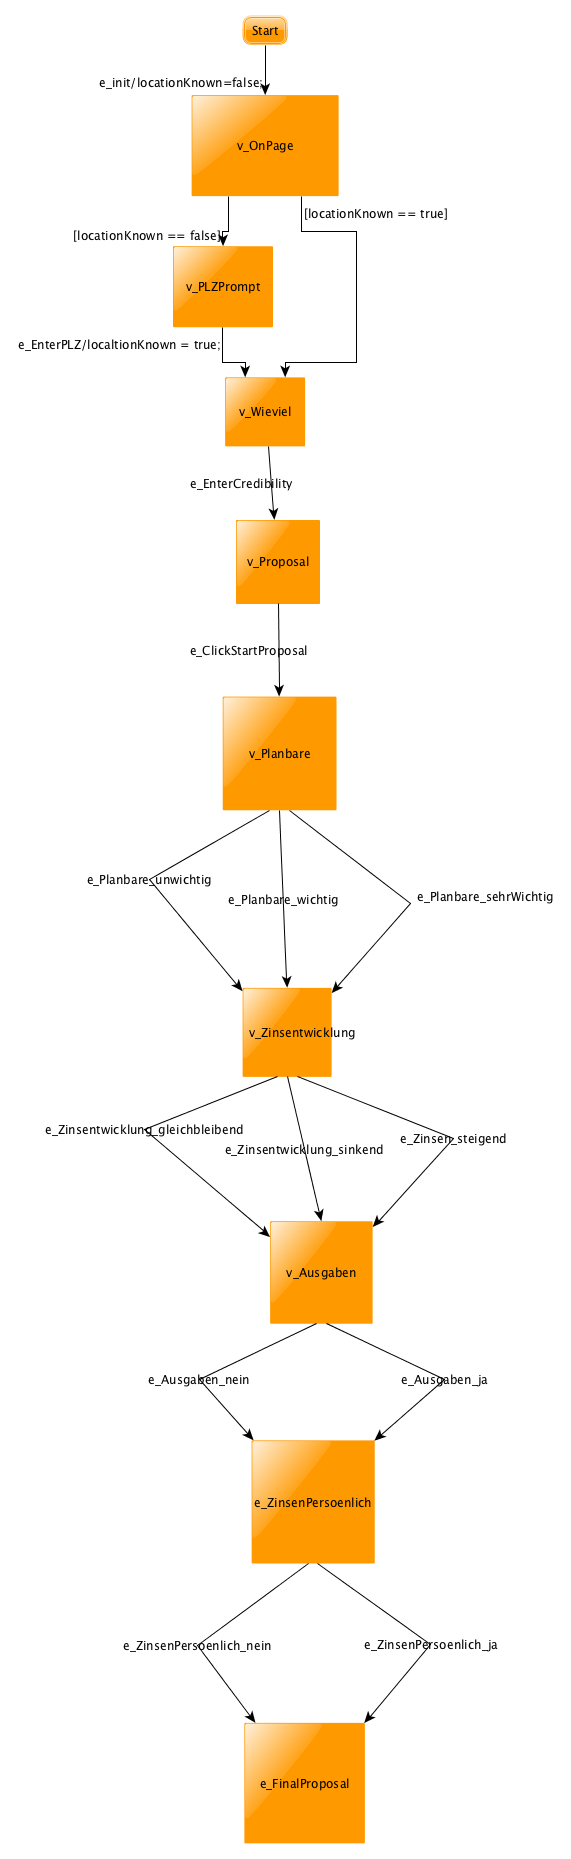
\includegraphics[width=0.45\textwidth]{figures/modell_abstract.png}
  \caption{}
  \label{fig:modell_abstract}
\end{figure}

\paragraph{Logik-Modellierung und Verfeinerung. Knoten: 72/51, Kanten: 72//66}
Bei der Logik-Modellierung wird das System nicht mehr als reine Blackbox gesehen. Das Modell soll weiterhin eine Abstraktion des SUT sein aber der Detailgrad erhöht sich. Dies hat zur Folge, dass zwar mehr Knoten und Kanten erstellt werden müssen, die Komplexität im Code sich aber verringert. Erreicht wird dies durch die explizite Modellierung von Kanten und Knoten mit identischen Bezeichnern. In diesem Beispiel, wo nur der Endzustand \texttt{v\_finalProposal} einer detaillierten Prüfung unterzogen wird, erhalten nur die Knoten auf unterster Ebene eindeutige Bezeichner. Graphwalker generiert nun zwar 36 Methoden(entsprechend den 36 Knoten mit den Bezeichnern \texttt{v\_finalProposalXX}, die dem Knoten \texttt{v\_finalProposal} aus dem Workflow-Modell entsprechen, aber diese enthalten keinerlei Logik um den Pfad zu reproduzieren. In diesen Methoden befindet sich also nur ein Bruchteil der Logik die im letzten Knoten der Workflow-Modellierung zu finden ist. Durch die explizite Modellierung aller möglichen Pfad ist implizit gegeben wie das SUT traversiert wurde und welche Prüflogik angewandt werden muss. Die Abbildung \ref{fig:modell_komplex} zeigt die logisch modellierte Variante des Hypothekarrechners.

\begin{figure}[h] 
  \centering
     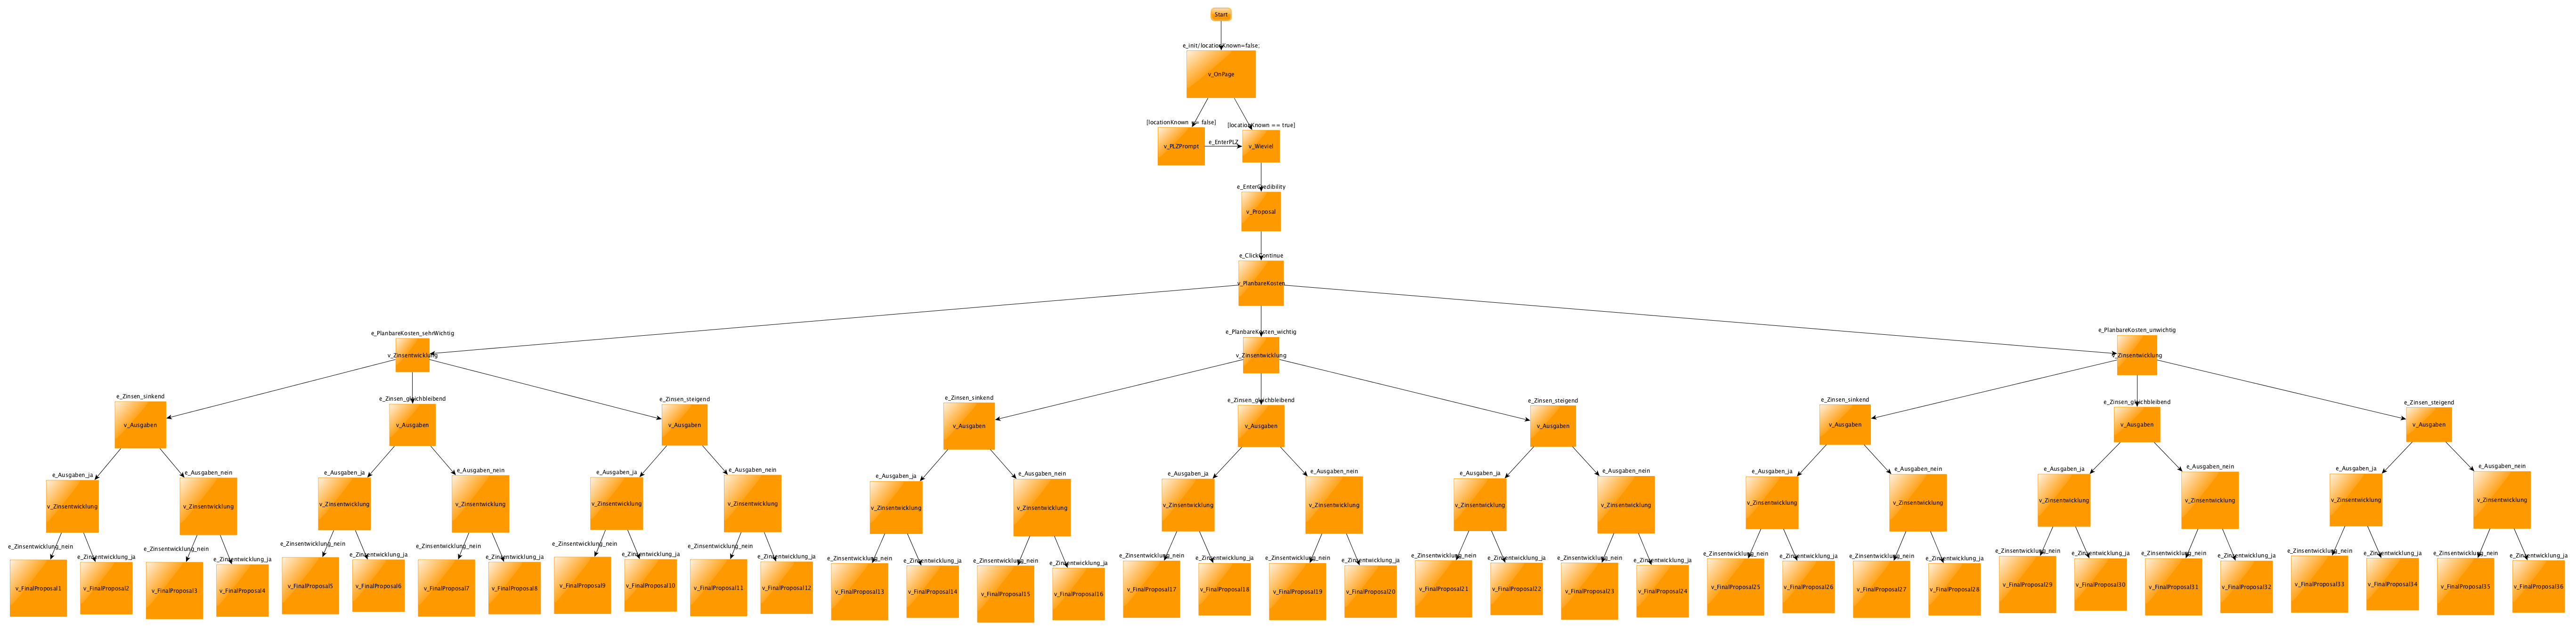
\includegraphics[width=1.5\textwidth, angle=90]{figures/modell_komplex.png}
  \caption{}
  \label{fig:modell_komplex}
\end{figure}

Es fällt schnell auf, dass das Hinzufügen von nur wenigen Mehroptionen im Prinzip das selbe, aus dem Model Checking bekannte, Problem der kombinatorischen Zustandsexplosion aufwirft\cite{clarke_model_2012}. Verglichen mit den Ansätzen aus diesem Feld (wie \textit{Counterexample-guided abstraction refinement}\cite{clarke_counterexample-guided_2000}), bei denen eine Abstraktion verfeinert wird, geht man hier aus der anderen Richtung vor. Man betrachtet die Programmlogik auf Code-Ebene genauer und versucht Abstraktionen des komplexen Modells zu generieren. Bei numerischen Werten können zum Beispiel weniger Werte modelliert werden (Konzentration auf Grenz- und Extremwerte). Beim Beispiel des Hypothekarrechners stellte sich heraus, dass die zugrundeliegende Programmlogik gar keine 36 Ergebniskategorien erzeugen kann. Die beiden letzten der vier Fragen generieren also keine eigene Ergebniskategorie sondern \textit{schieben} das Ergebnis in eine der anderen Kategorien. Gezeigt wird diese vereinfachte Version des Modells in Abbildung \ref{fig:modell_logisch}. Gut zu sehen sind die Überschneidungen auf zweitletzter Ebene die zu deutlich weniger Endzuständen und damit zu weniger Code führen.\\
Durch eine verstärkte Whitebox-Ansicht muss der Modellierer also versuchen die  Zustände und Übergänge im Modell zu verringern.


\begin{figure}[h] 
  \centering
     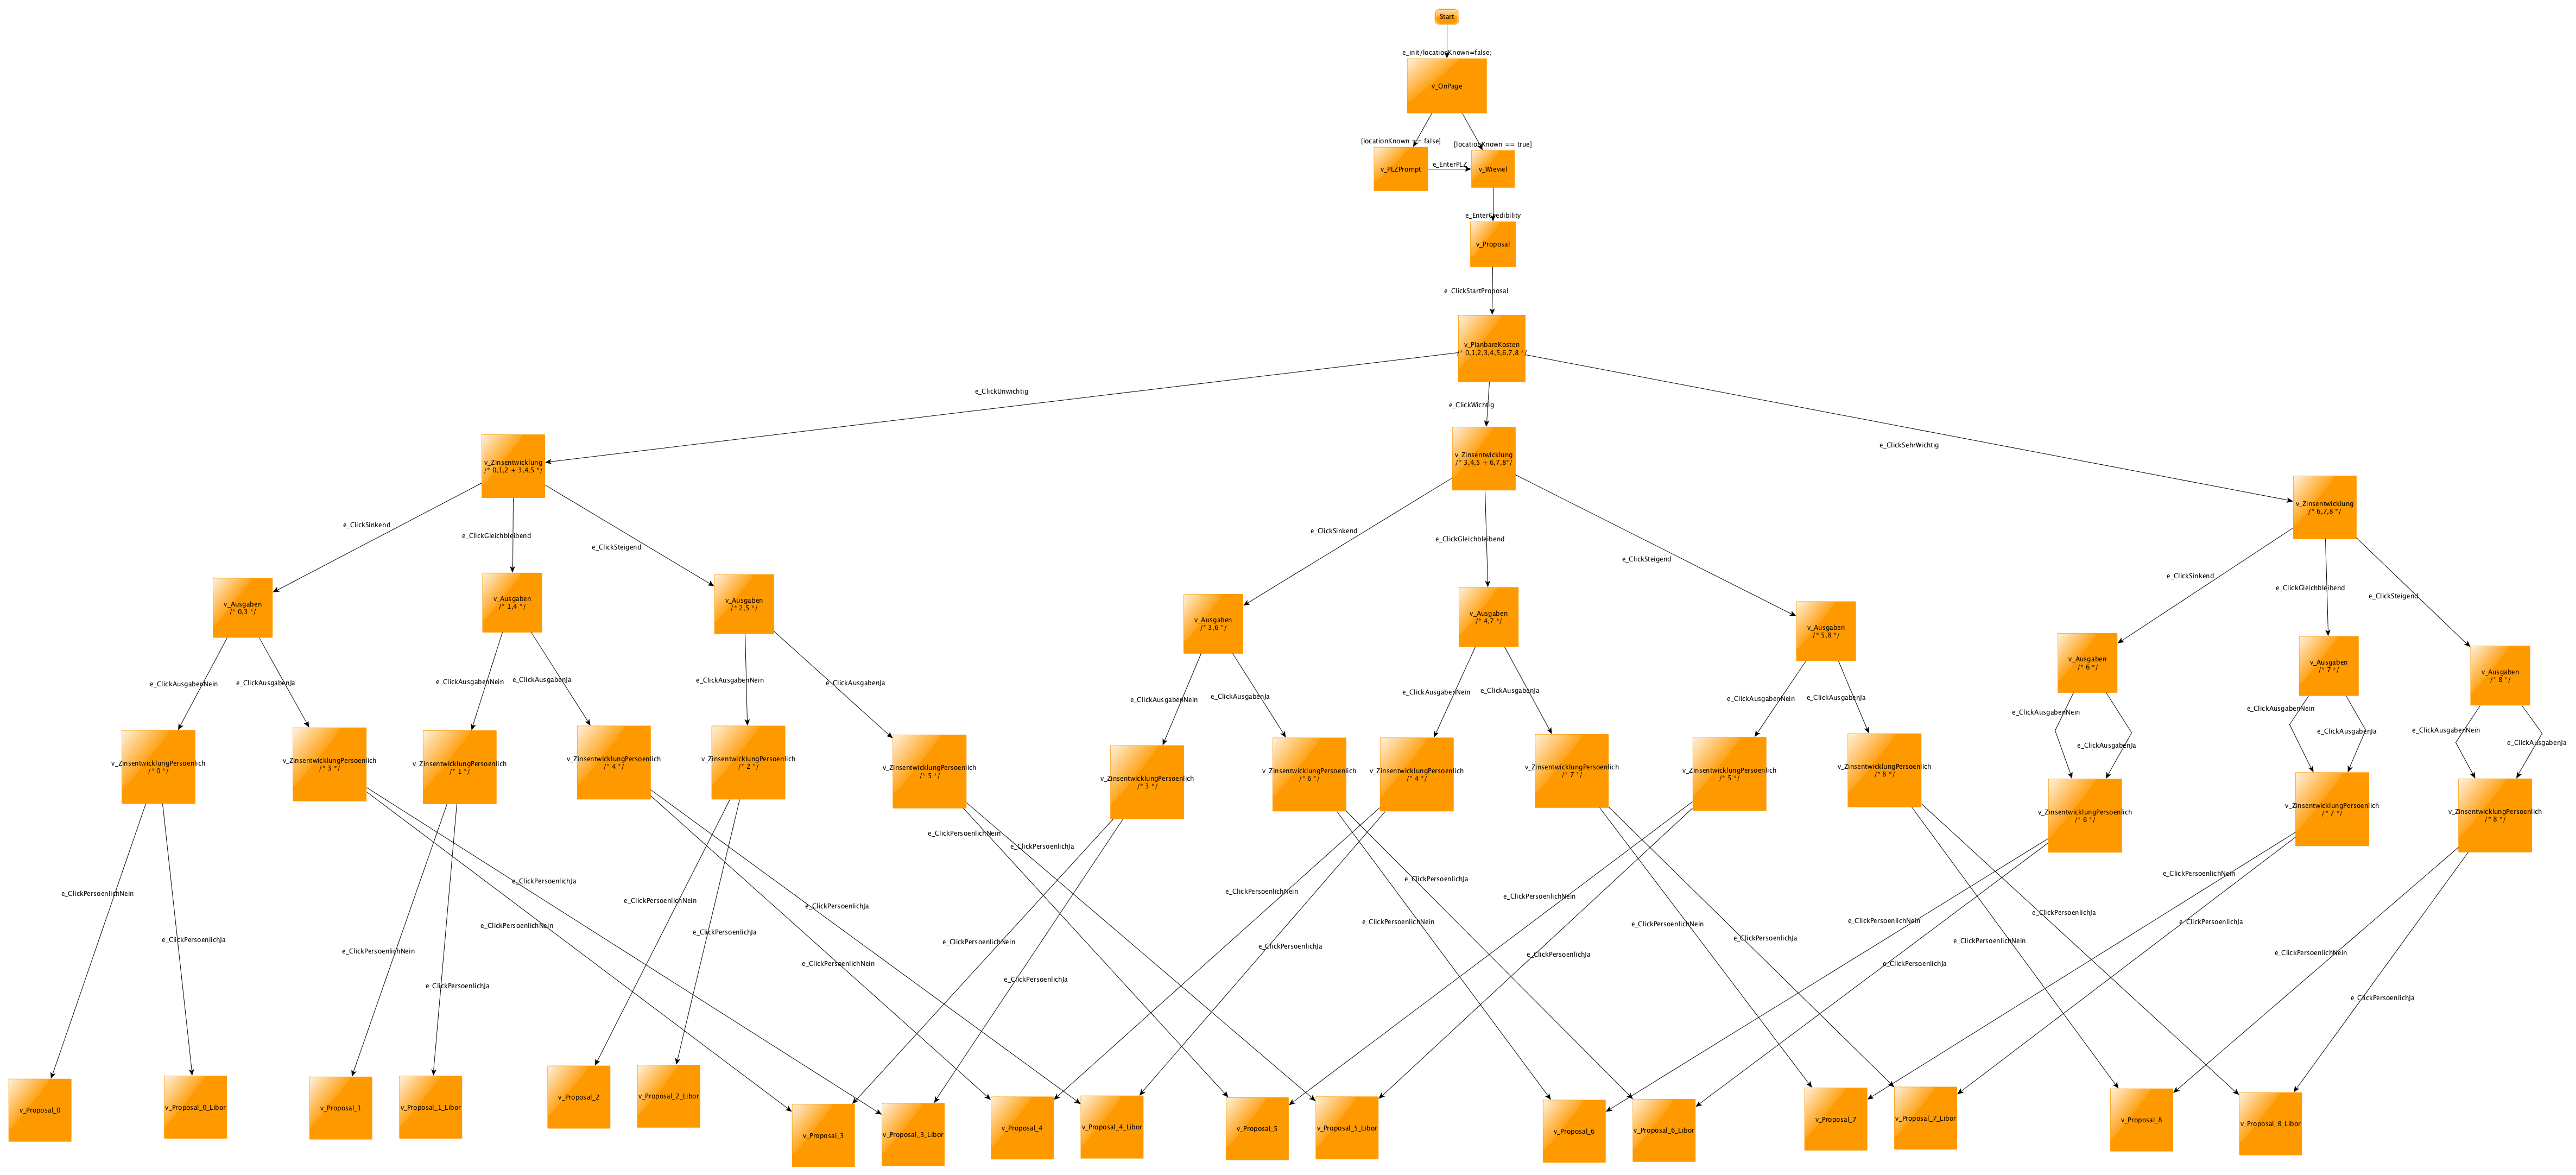
\includegraphics[width=1.5\textwidth, angle=90]{figures/modell_logisch.png}
  \caption{}
  \label{fig:modell_logisch}
\end{figure}

\paragraph{Modellbasierte Tests auf niedrigeren Ebenen} Dieses Beispiel zeigte die Mächtigkeit von Graphwalker in Verbindung mit einem Framework für das GUI-Testing. Statt eines GUI-Testing-Frameworks können aber beliebige andere Frameworks für den Adapter-Code verwendet werden. Damit wird das Testing auch auf Schnittstellen- und Unit-Testebene möglich. In Verbindung mit einer sinnvollen Testing API zum SUT, können aber genauso Tests der Businesslogik modelliert werden. Also eine Art Unit-Test aus Sicht des Fachbereichs in Form eines Modells. Denkbar sind Abläufe wie das Laden eines Kunden, die Modifikation seiner Stammdaten und die abschließende Überprüfung ob diese Modifikationen fehlerfrei abgelegt wurden. Die Modelle lassen eine unbegrenzte Komplexität zu. Seltene, lange aber geschäftskritische Workflows lassen sich damit sehr gut darstellen.

\section{Zugewinne durch die Kombination von BDD und MBT}
Gerade für die agile Entwicklung ist die Kombination von BDD und MBT wie maßgeschneidert. Agile Entwicklung bedeutet unter anderem viel Kontakt mit dem Kunden und damit auch die Notwendigkeit der Auseinandersetzung mit Spezifikationen und Feedback. CoS-artige Definitionen kommen in vielen Softwareprojekten bereits zum Einsatz und sind daher sowohl dem fachlichen als auch dem technischen Personal bekannt. Der Schritt von CoS-Tabellen zu BDD-Testfällen, egal welches Framework dazu benutzt wird, ist schmerzlos. Wenn der Einsatz von BDD-Tests sorgfältig und gut koordiniert umgesetzt wird, ist die damit einhergehende Versionierung der CoS ein wertvoller Nebeneffekt der die Organisation des Softwareprojekts vereinfacht.\\
Eine ähnliche Kombination von Methoden schlägt auch Binder vor\cite{binder_model-based_2014}. Er warnt aber davor, dass BDD nur einen kleinen Teil des \textit{happy-path} abdecken. Soll heißen, dass das System mittels CoS nur auf sehr wenigen Pfaden getestet wird. Außerdem wächst die Anzahl der zu wartenden BDD-Spezifikationen mit der Größe der Code-Basis. Meist hat dies zur Folge, dass ältere Spezifikationen in Vergessenheit geraten und nicht mehr in das Regressionstesting miteinbezogen werden. Um zweiterem Nachteil entgegenzuwirken müssen BDD-Spezifikationen sehr sorgfältig und mit Hinblick auf die Programmlogik entworfen werden. Außerdem muss die Versionierung Team-übergreifend nahtlos funktionieren.\\
Aus Kundensicht sind CoS oft notwendig, da sie kurz und bündig vertraglich festgehalten werden können. Wenn der Kunde beim Abnahmetest auf CoS Spezifikationen besteht, muss das System trotzdem durch breitere Maßnahmen regressiv getestet werden. Hier ergänzen modellbasierte Tests die Qualitätssicherungsmaßnahmen. Ein CoS kann als einzelner Pfad in einem Modell gesehen werden. Der modellbasierte Test prüft dann, mit variablem Grad an Assertions, alle anderen Pfade. Diese Vorgehensweise schafft eine weitere Schicht an Sicherheit und lässt sich gut in bestehende Projekt- und Softwarestrukturen integrieren.













